% Unit: AP CSP sample exam questions (College Board style).
% Place image files under \texttt{exam-test/cs-p/images/} using the basenames below (e.g.\ \texttt{.png} or \texttt{.pdf}).
% Load after \texttt{cs-p/01-practice.tex}, which must contain exactly 42 questions, so numbering continues (43--64).

\runningheader{Computer Science Principles}{AP Practice Exam (Set 2)}{Page \thepage\ of \numpages}

\begingradingrange{csp2}

\question[5]
A video-streaming Web site uses 32-bit integers to count the number of times each video has been played. In anticipation of some videos being played more times than can be represented with 32 bits, the Web site is planning to change to 64-bit integers for the counter. Which of the following best describes the result of using 64-bit integers instead of 32-bit integers?
\begin{choices}
  \choice 2 times as many values can be represented. 
  \choice 32 times as many values can be represented.
  \CorrectChoice $2^{32}$ times as many values can be represented.
  \choice $32^{2}$ times as many values can be represented.
\end{choices}
\begin{solution}
  Unsigned range doubles with each bit; increasing width by 32 bits multiplies representable values by $2^{32}$.
\end{solution}

\question[5]
A programmer completes the user manual for a video game she has developed and realizes she has reversed the roles of goats and sheep throughout the text. Consider the programmer's goal of changing all occurrences of ``goats'' to ``sheep'' and all occurrences of ``sheep'' to ``goats.'' The programmer will use the fact that the word ``foxes'' does not appear anywhere in the original text.

Which of the following algorithms can be used to accomplish the programmer's goal?
\begin{choices}
  \choice First, change all occurrences of ``goats'' to ``sheep.'' Then, change all occurrences of ``sheep'' to ``goats.''
  \choice First, change all occurrences of ``goats'' to ``sheep.'' Then, change all occurrences of ``sheep'' to ``goats.'' Last, change all occurrences of ``foxes'' to ``sheep.''
  \CorrectChoice First, change all occurrences of ``goats'' to ``foxes.'' Then, change all occurrences of ``sheep'' to ``goats.'' Last, change all occurrences of ``foxes'' to ``sheep.''
  \choice First, change all occurrences of ``goats'' to ``foxes.'' Then, change all occurrences of ``foxes'' to ``sheep.'' Last, change all occurrences of ``sheep'' to ``goats.''
\end{choices}
\begin{solution}
  Use a temporary token (\texttt{foxes}) so no intermediate step overwrites text still needed for a later replacement.
\end{solution}

\newpage

\question[5]
ASCII is a character-encoding scheme that uses a numeric value to represent each character. For example, the uppercase letter ``G'' is represented by the decimal (base 10) value 71. A partial list of characters and their corresponding ASCII values is shown below.
\begin{center}
  \small
  \begin{tabular}{|c|c|c|c|c|c|c|c|}
    \hline
    Dec. & Char & Dec. & Char & Dec. & Char & Dec. & Char \\
    \hline
    65 & A & 73 & I & 81 & Q & 89 & Y \\
    \hline
    66 & B & 74 & J & 82 & R & 90 & Z \\
    \hline
    67 & C & 75 & K & 83 & S & & \\
    \hline
    68 & D & 76 & L & 84 & T & & \\
    \hline
    69 & E & 77 & M & 85 & U & & \\
    \hline
    70 & F & 78 & N & 86 & V & & \\
    \hline
    71 & G & 79 & O & 87 & W & & \\
    \hline
    72 & H & 80 & P & 88 & X & & \\
    \hline
  \end{tabular}
\end{center}
ASCII characters can also be represented by hexadecimal numbers. According to ASCII character encoding, which of the following letters is represented by the hexadecimal (base 16) number \texttt{56}?
\begin{choices}
  \choice A
  \choice L
  \CorrectChoice V
  \choice Y
\end{choices}
\begin{solution}
  $0\text{x}56 = 5\cdot 16 + 6 = 86$, which is ASCII ``V''.
\end{solution}

\newpage

\question[5]
The figure below shows a circuit composed of two logic gates. The output of the circuit is true.
\begin{center}
  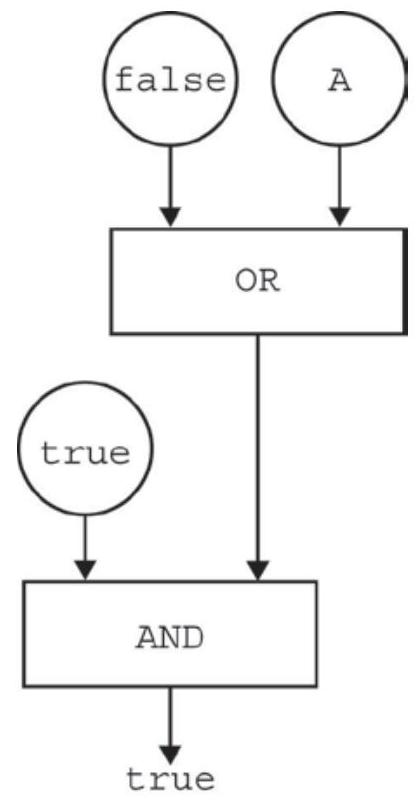
\includegraphics[width=0.30\linewidth]{cs-p/images/68b75e92-b243-4d72-a2a7-db8b0e1b4bf4-04_802_418_380_850}
\end{center}

Which of the following is a true statement about input A?
\begin{choices}
  \CorrectChoice Input A must be true.
  \choice Input A must be false.
  \choice Input A can be either true or false.
  \choice There is no possible value of input $A$ that will cause the circuit to have the output true.
\end{choices}
\begin{solution}
  Original answer key: A (trace gates using the diagram).
\end{solution}

\newpage

\question[5]
The following question uses a robot in a grid of squares. The robot is represented as a triangle, which is initially in the bottom left square of the grid and facing right.
\begin{center}
  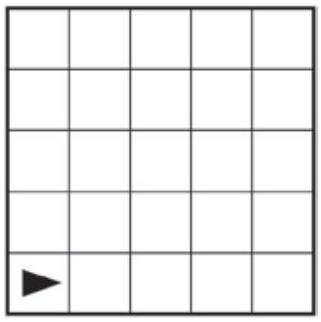
\includegraphics[width=0.35\linewidth]{cs-p/images/68b75e92-b243-4d72-a2a7-db8b0e1b4bf4-05_322_321_433_902}
\end{center}

Consider the following code segment, which moves the robot in the grid.
\begin{center}
  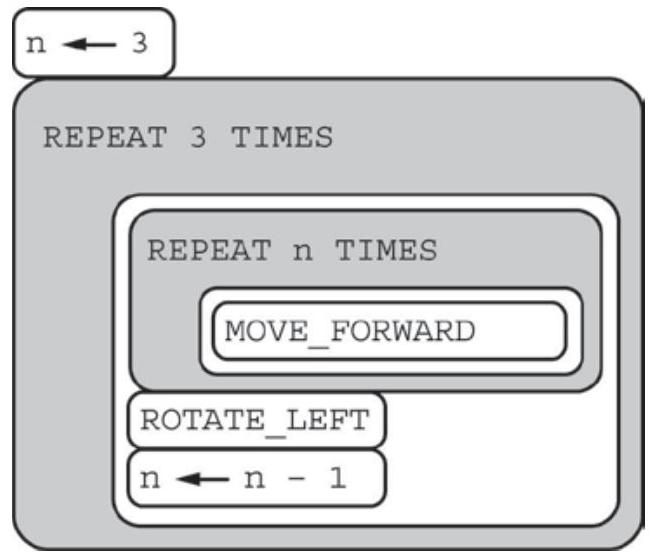
\includegraphics[width=0.35\linewidth]{cs-p/images/68b75e92-b243-4d72-a2a7-db8b0e1b4bf4-05_558_652_863_734}
\end{center}

Which of the following shows the location of the robot after running the code segment?
\begin{center}
  \begin{minipage}[t]{0.24\linewidth}\centering
    \textbf{(A)}\\[0.5em]
    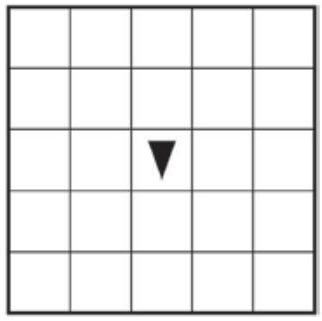
\includegraphics[width=\linewidth]{cs-p/images/68b75e92-b243-4d72-a2a7-db8b0e1b4bf4-05_321_322_1512_433}
  \end{minipage}\hfill
  \begin{minipage}[t]{0.24\linewidth}\centering
    \textbf{(B)}\\[0.5em]
    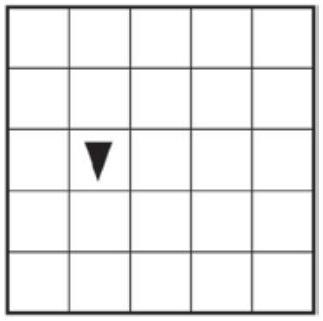
\includegraphics[width=\linewidth]{cs-p/images/68b75e92-b243-4d72-a2a7-db8b0e1b4bf4-05_321_323_1512_1194}
  \end{minipage}
  \begin{minipage}[t]{0.24\linewidth}\centering
    \textbf{(C)}\\[0.5em]
    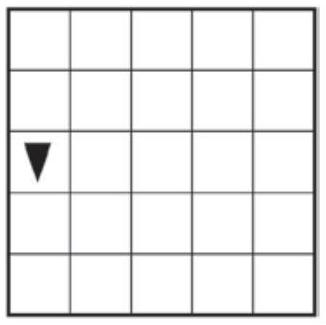
\includegraphics[width=\linewidth]{cs-p/images/68b75e92-b243-4d72-a2a7-db8b0e1b4bf4-05_325_326_1916_433}
  \end{minipage}\hfill
  \begin{minipage}[t]{0.24\linewidth}\centering
    \textbf{(D)}\\[0.5em]
    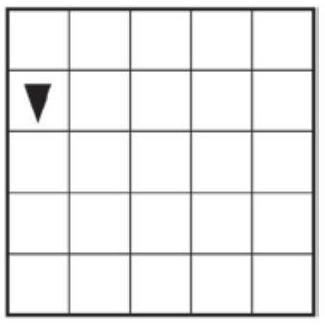
\includegraphics[width=\linewidth]{cs-p/images/68b75e92-b243-4d72-a2a7-db8b0e1b4bf4-05_325_325_1916_1194}
  \end{minipage}
\end{center}
\begin{choices}
  \CorrectChoice (A)
  \choice (B)
  \choice (C)
  \choice (D)
\end{choices}
\begin{solution}
  Original answer key: A.
\end{solution}

\question[5]
Which of the following statements describes a limitation of using a computer simulation to model a real-world object or system?
\begin{choices}
  \choice Computer simulations can only be built after the real-world object or system has been created.
  \choice Computer simulations only run on very powerful computers that are not available to the general public.
  \CorrectChoice Computer simulations usually make some simplifying assumptions about the real-world object or system being modeled.
  \choice It is difficult to change input parameters or conditions when using computer simulations.
\end{choices}
\begin{solution}
  Models omit detail by design; that is a core limitation of simulation.
\end{solution}


\question[5]
A certain social media Web site allows users to post messages and to comment on other messages that have been posted. When a user posts a message, the message itself is considered data. In addition to the data, the site stores the following metadata.
\begin{itemize}
  \item The time the message was posted
  \item The name of the user who posted the message
  \item The names of any users who comment on the message and the times the comments were made
\end{itemize}
For which of the following goals would it be more useful to analyze the \textbf{data} instead of the metadata?
\begin{choices}
  \choice To determine the users who post messages most frequently
  \choice To determine the time of day that the site is most active
  \CorrectChoice To determine the topics that many users are posting about
  \choice To determine which posts from a particular user have received the greatest number of comments
\end{choices}
\begin{solution}
  Topics are inferred from message \emph{content} (data), not from timestamps or names alone.
\end{solution}

\newpage

\question[5]
The program segment below is intended to move a robot in a grid to a gray square. The program segment uses the procedure \texttt{GoalReached}, which evaluates to true if the robot is in the gray square and evaluates to false otherwise. The robot in each grid is represented as a triangle and is initially facing left. The robot can move into a white or gray square but cannot move into a black region.
\begin{lstlisting}[style=pseudo]
REPEAT UNTIL (GoalReached ())
{
    IF (CAN_MOVE (forward))
    {
        MOVE_FORWARD ()
    }
    IF (CAN_MOVE (right))
    {
        ROTATE_RIGHT ()
    }
    IF (CAN_MOVE (left))
    {
        ROTATE_LEFT ()
    }
}
\end{lstlisting}
For which of the following grids does the program \textbf{not} correctly move the robot to the gray square?
\begin{center}
  \begin{minipage}[t]{0.24\linewidth}\centering
    \textbf{(A)}\\[0.4em]
    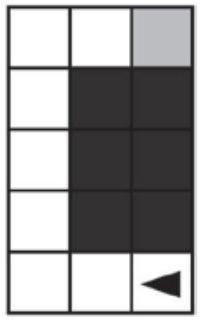
\includegraphics[width=\linewidth]{cs-p/images/68b75e92-b243-4d72-a2a7-db8b0e1b4bf4-08_321_201_416_433}
  \end{minipage}\hfill
  \begin{minipage}[t]{0.24\linewidth}\centering
    \textbf{(B)}\\[0.4em]
    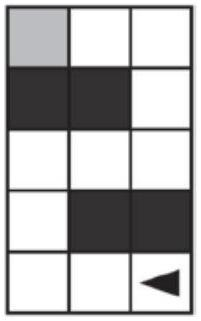
\includegraphics[width=\linewidth]{cs-p/images/68b75e92-b243-4d72-a2a7-db8b0e1b4bf4-08_321_201_416_1194}
  \end{minipage}
  \begin{minipage}[t]{0.24\linewidth}\centering
    \textbf{(C)}\\[0.4em]
    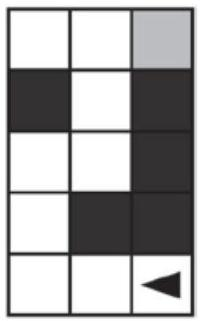
\includegraphics[width=\linewidth]{cs-p/images/68b75e92-b243-4d72-a2a7-db8b0e1b4bf4-08_321_201_820_433}
  \end{minipage}\hfill
  \begin{minipage}[t]{0.24\linewidth}\centering
    \textbf{(D)}\\[0.4em]
    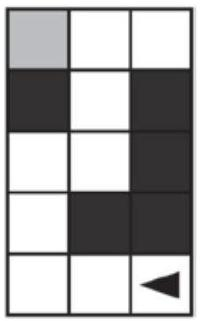
\includegraphics[width=\linewidth]{cs-p/images/68b75e92-b243-4d72-a2a7-db8b0e1b4bf4-08_321_201_820_1194}
  \end{minipage}
\end{center}
\begin{choices}
  \choice (A)
  \choice (B)
  \choice (C)
  \CorrectChoice (D)
\end{choices}
\begin{solution}
  Original answer key: D.
\end{solution}

\newpage

\question[5]
The table below shows the time a computer system takes to complete a specified task on the customer data of different-sized companies.
\begin{center}
  \small
  \begin{tabular}{|l|c|c|c|}
    \hline
    Task & Small ($\approx$100) & Medium ($\approx$1,000) & Large ($\approx$10,000) \\
    \hline
    Backing up data & 2 h & 20 h & 200 h \\
    \hline
    Deleting entries from data & 100 h & 200 h & 300 h \\
    \hline
    Searching through data & 250 h & 300 h & 350 h \\
    \hline
    Sorting data & 0.01 h & 1 h & 100 h \\
    \hline
  \end{tabular}
\end{center}
Based on the information in the table, which of the following tasks is likely to take the \textbf{longest} amount of time when scaled up for a very large company of approximately 100,000 customers?
\begin{choices}
  \choice Backing up data
  \choice Deleting entries from data
  \choice Searching through data
  \CorrectChoice Sorting data
\end{choices}
\begin{solution}
  Sorting grows much faster with $n$ than the other tasks shown; original answer key: D.
\end{solution}

\question[5]
Consider the code segment below. If the variables \texttt{onTime} and \texttt{absent} both have the value \texttt{false}, what is displayed as a result of running the code segment?
\begin{center}
  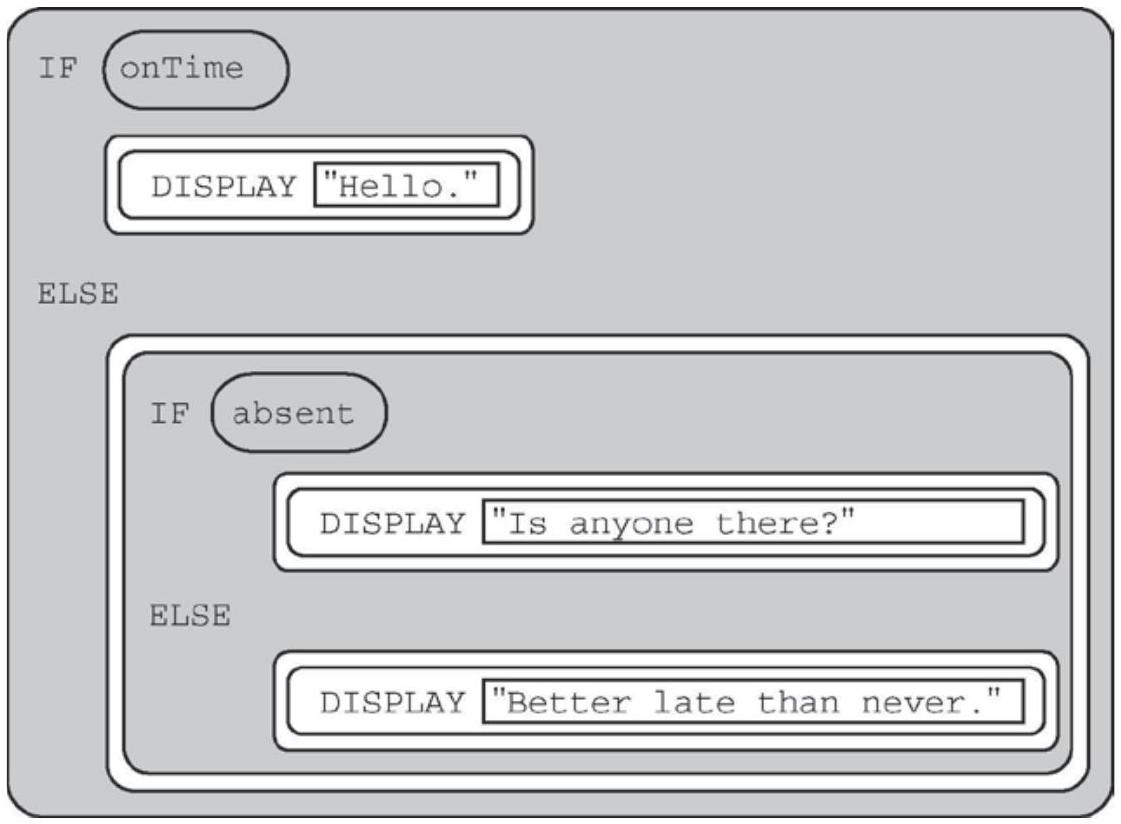
\includegraphics[width=0.35\linewidth]{cs-p/images/68b75e92-b243-4d72-a2a7-db8b0e1b4bf4-09_824_1121_1194_502}
\end{center}
\begin{choices}
  \choice \texttt{Is anyone there?}
  \CorrectChoice \texttt{Better late than never.}
  \choice \texttt{Hello. Is anyone there?}
  \choice \texttt{Hello. Better late than never.}
\end{choices}
\begin{solution}
  Original answer key: B (follow branches in the diagram).
\end{solution}

\newpage

\question[5]
Under which of the following conditions is it most beneficial to use a heuristic approach to solve a problem?
\begin{choices}
  \choice When the problem can be solved in a reasonable time and an approximate solution is acceptable
  \choice When the problem can be solved in a reasonable time and an exact solution is needed
  \CorrectChoice When the problem cannot be solved in a reasonable time and an approximate solution is acceptable
  \choice When the problem cannot be solved in a reasonable time and an exact solution is needed
\end{choices}
\begin{solution}
  Heuristics trade optimality (or certainty) for feasible runtime.
\end{solution}

\question[5]
Which of the following are true statements about digital certificates in Web browsers?

\textbf{I.} Digital certificates are used to verify the ownership of encrypted keys used in secured communication.

\textbf{II.} Digital certificates are used to verify that the connection to a Web site is fault tolerant.
\begin{choices}
  \CorrectChoice I only
  \choice II only
  \choice I and II
  \choice Neither I nor II
\end{choices}
\begin{solution}
  Certificates bind identities to public keys; they do not by themselves guarantee fault tolerance.
\end{solution}

\newpage

\question[5]
There are 32 students standing in a classroom. Two different algorithms are given for finding the average height of the students.

\textbf{Algorithm A}

Step 1: All students stand.

Step 2: A randomly selected student writes his or her height on a card and is seated.

Step 3: A randomly selected standing student adds his or her height to the value on the card, records the new value on the card, and is seated. The previous value on the card is erased.

Step 4: Repeat step 3 until no students remain standing.

Step 5: The sum on the card is divided by 32. The result is given to the teacher.

\textbf{Algorithm B}

Step 1: All students stand.

Step 2: Each student is given a card. Each student writes his or her height on the card.

Step 3: Standing students form random pairs at the same time. Each pair adds the numbers written on their cards and writes the result on one student's card; the other student is seated. The previous value on the card is erased.

Step 4: Repeat step 3 until one student remains standing.

Step 5: The sum on the last student's card is divided by 32. The result is given to the teacher.

Which of the following statements is true?
\begin{choices}
  \choice Algorithm A always calculates the correct average, but Algorithm B does not.
  \choice Algorithm B always calculates the correct average, but Algorithm A does not.
  \CorrectChoice Both Algorithm A and Algorithm B always calculate the correct average.
  \choice Neither Algorithm A nor Algorithm B calculates the correct average.
\end{choices}
\begin{solution}
  Both accumulate the sum of all heights (commutative addition); dividing by 32 yields the mean.
\end{solution}


\newpage

\question[5]
The figure below shows a robot in a grid of squares. The robot is represented as a triangle, which is initially facing upward. The robot can move into a white or gray square but cannot move into a black region.
\begin{center}
  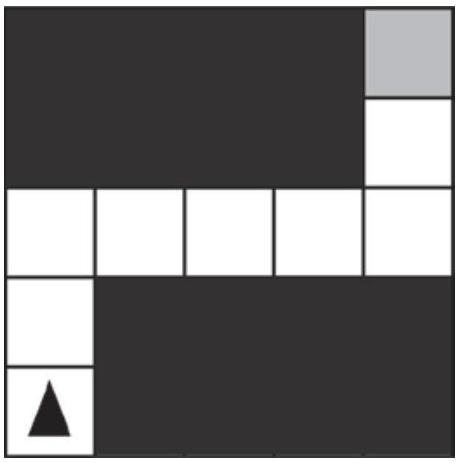
\includegraphics[width=0.35\linewidth]{cs-p/images/68b75e92-b243-4d72-a2a7-db8b0e1b4bf4-12_463_461_476_833}
\end{center}

Consider the procedure \texttt{MoveAndTurn} below.
\begin{center}
  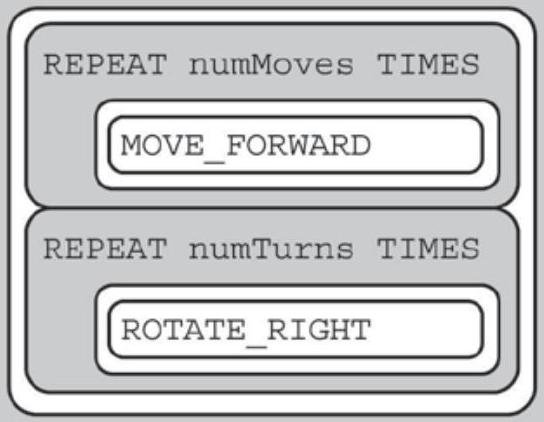
\includegraphics[width=0.35\linewidth]{cs-p/images/68b75e92-b243-4d72-a2a7-db8b0e1b4bf4-12_422_544_1162_700}
\end{center}

Which of the following code segments will move the robot to the gray square?
\begin{center}
  \begin{minipage}[t]{0.24\linewidth}\centering
    \textbf{(A)}\\[0.4em]
    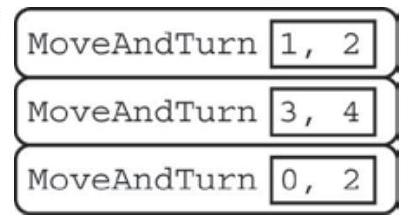
\includegraphics[width=\linewidth]{cs-p/images/68b75e92-b243-4d72-a2a7-db8b0e1b4bf4-12_222_409_1697_423}
  \end{minipage}\hfill
  \begin{minipage}[t]{0.24\linewidth}\centering
    \textbf{(B)}\\[0.4em]
    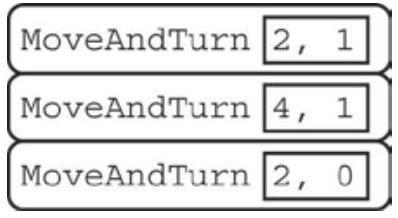
\includegraphics[width=\linewidth]{cs-p/images/68b75e92-b243-4d72-a2a7-db8b0e1b4bf4-12_218_398_1701_1190}
  \end{minipage}
  \begin{minipage}[t]{0.24\linewidth}\centering
    \textbf{(C)}\\[0.4em]
    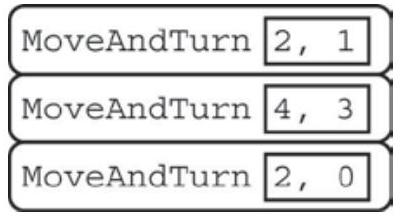
\includegraphics[width=\linewidth]{cs-p/images/68b75e92-b243-4d72-a2a7-db8b0e1b4bf4-12_218_403_2015_429}
  \end{minipage}\hfill
  \begin{minipage}[t]{0.24\linewidth}\centering
    \textbf{(D)}\\[0.4em]
    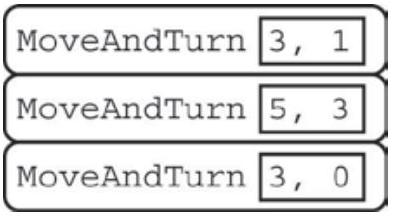
\includegraphics[width=\linewidth]{cs-p/images/68b75e92-b243-4d72-a2a7-db8b0e1b4bf4-12_218_394_2015_1194}
  \end{minipage}
\end{center}
\begin{choices}
  \choice Choice \textbf{(A)}
  \choice Choice \textbf{(B)}
  \CorrectChoice Choice \textbf{(C)}
  \choice Choice \textbf{(D)}
\end{choices}
\begin{solution}
  Original answer key: C.
\end{solution}

\newpage

\question[5]
Biologists often attach tracking collars to wild animals. For each animal, the following geolocation data is collected at frequent intervals.
\begin{itemize}
  \item The time
  \item The date
  \item The location of the animal
\end{itemize}
Which of the following questions about a particular animal could \textbf{not} be answered using only the data collected from the tracking collars?
\begin{choices}
  \choice Approximately how many miles did the animal travel in one week?
  \choice Does the animal travel in groups with other tracked animals?
  \CorrectChoice Do the movement patterns of the animal vary according to the weather?
  \choice In what geographic locations does the animal typically travel?
\end{choices}
\begin{solution}
  Weather observations are not in the collar data set; original answer key: C.
\end{solution}

\question[5]
A summer camp offers a morning session and an afternoon session. The list \texttt{morningList} contains the names of all children attending the morning session, and the list \texttt{afternoonList} contains the names of all children attending the afternoon session.

Only children who attend \textbf{both} sessions eat lunch at the camp. The camp director wants to create \texttt{lunchList}, which will contain the names of children attending both sessions.

The following code segment is intended to create \texttt{lunchList}, which is initially empty. It uses the procedure \texttt{IsFound(list, name)}, which returns \texttt{true} if \texttt{name} is found in \texttt{list} and returns \texttt{false} otherwise.
\begin{lstlisting}[style=pseudo]
FOR EACH child IN morningList
{
    <MISSING CODE>
}
\end{lstlisting}
Which of the following could replace \texttt{<MISSING CODE>} so that the code segment works as intended?
\begin{choices}
  \CorrectChoice \texttt{IF (IsFound(afternoonList, child)) \{ APPEND(lunchList, child) \}}
  \choice \texttt{IF (IsFound(lunchList, child)) \{ APPEND(afternoonList, child) \}}
  \choice \texttt{IF (IsFound(morningList, child)) \{ APPEND(lunchList, child) \}}
  \choice \parbox[t]{0.92\linewidth}{\ttfamily IF ((IsFound(morningList, child)) OR (IsFound(afternoonList, child))) \{ APPEND(lunchList, child) \}}
\end{choices}
\begin{solution}
  Keep a child when they appear in both lists---check afternoon for each morning attendee; original answer key: A.
\end{solution}

\newpage

\question[5]
Consider the following program code.
\begin{center}
  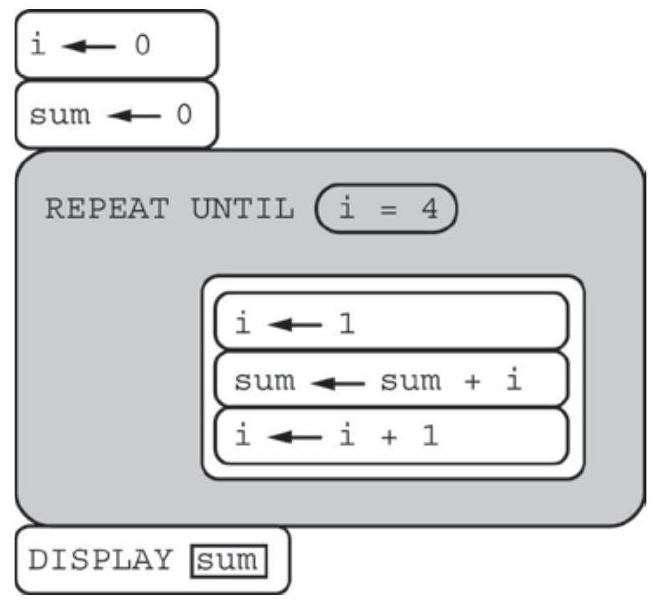
\includegraphics[width=0.35\linewidth]{cs-p/images/68b75e92-b243-4d72-a2a7-db8b0e1b4bf4-15_602_656_382_732}
\end{center}

Which of the following best describes the result of running the program code?
\begin{choices}
  \choice The number 0 is displayed.
  \choice The number 6 is displayed.
  \choice The number 10 is displayed.
  \CorrectChoice Nothing is displayed; the program results in an infinite loop.
\end{choices}
\begin{solution}
  Original answer key: D (trace the loop/update in the figure).
\end{solution}


\question[5]
Which of the following is a true statement about data compression?
\begin{choices}
  \choice Data compression is only useful for files being transmitted over the Internet.
  \choice Regardless of the compression technique used, once a data file is compressed, it cannot be restored to its original state.
  \choice Sending a compressed version of a file ensures that the contents of the file cannot be intercepted by an unauthorized user.
  \CorrectChoice There are trade-offs involved in choosing a compression technique for storing and transmitting data.
\end{choices}
\begin{solution}
  Lossless vs.\ lossy and speed/size trade-offs are inherent; original answer key: D.
\end{solution}

\newpage


\question[5]
An office building has two floors. A computer program is used to control an elevator that travels between the two floors. Physical sensors are used to set the following Boolean variables.
\begin{center}
  \small
  \begin{tabular}{|l|p{0.62\linewidth}|}
    \hline
    Variable & Description \\
    \hline
    \texttt{onFloor1} & \texttt{true} if the elevator is stopped on floor 1; otherwise \texttt{false} \\
    \hline
    \texttt{onFloor2} & \texttt{true} if the elevator is stopped on floor 2; otherwise \texttt{false} \\
    \hline
    \texttt{callTo1} & \texttt{true} if the elevator is called to floor 1; otherwise \texttt{false} \\
    \hline
    \texttt{callTo2} & \texttt{true} if the elevator is called to floor 2; otherwise \texttt{false} \\
    \hline
  \end{tabular}
\end{center}
The elevator moves when the door is closed and the elevator is called to the floor that it is not currently on. Which of the following Boolean expressions can be used in a selection statement to cause the elevator to move?
\begin{choices}
  \choice $(\texttt{onFloor1} \textbf{ AND } \texttt{callTo2}) \textbf{ AND } (\texttt{onFloor2} \textbf{ AND } \texttt{callTo1})$
  \CorrectChoice $(\texttt{onFloor1} \textbf{ AND } \texttt{callTo2}) \textbf{ OR } (\texttt{onFloor2} \textbf{ AND } \texttt{callTo1})$
  \choice $(\texttt{onFloor1} \textbf{ OR } \texttt{callTo2}) \textbf{ AND } (\texttt{onFloor2} \textbf{ OR } \texttt{callTo1})$
  \choice $(\texttt{onFloor1} \textbf{ OR } \texttt{callTo2}) \textbf{ OR } (\texttt{onFloor2} \textbf{ OR } \texttt{callTo1})$
\end{choices}
\begin{solution}
  Move when on floor 1 and called to 2, or on floor 2 and called to 1; original answer key: B.
\end{solution}

\question[5]
According to the domain name system (DNS), which of the following is a subdomain of the domain \texttt{example.com}?
\begin{choices}
  \CorrectChoice \texttt{about.example.com}
  \choice \texttt{example.co.uk}
  \choice \texttt{example.com.org}
  \choice \texttt{example.org}
\end{choices}
\begin{solution}
  \texttt{about} is a subdomain label of \texttt{example.com}; original answer key: A.
\end{solution}

\newpage


\question[5]
Which of the following algorithms require both \textbf{selection} and \textbf{iteration}?

\textbf{Select two answers.}
\begin{checkboxes}
  \choice An algorithm that, given two integers, displays the greater of the two integers
  \CorrectChoice An algorithm that, given a list of integers, displays the number of even integers in the list
  \CorrectChoice An algorithm that, given a list of integers, displays only the negative integers in the list
  \choice An algorithm that, given a list of integers, displays the sum of the integers in the list
\end{checkboxes}
\begin{solution}
  Counting evens and filtering negatives need loops and conditionals; original answer key: B and C.
\end{solution}

\question[5]
A teacher uses the following program to adjust student grades on an assignment by adding 5 points to each student's original grade. However, if adding 5 points causes a grade to exceed 100 points, the student receives a score of 100 points. The students' original grades are stored in the list \texttt{gradeList}, which is indexed from 1 to $n$.

The teacher has procedures $\min(a,b)$ and $\max(a,b)$ as usual.

\begin{lstlisting}[style=pseudo]
i <- 1
REPEAT n TIMES
{
    <MISSING CODE>
    i <- i + 1
}
\end{lstlisting}

Which of the following code segments can replace \texttt{<MISSING CODE>} so that the program works as intended?

\textbf{Select two answers.}
\begin{checkboxes}
  \CorrectChoice \texttt{gradeList[i] <- min(gradeList[i] + 5, 100)}
  \choice \texttt{gradeList[i] <- max(gradeList[i] + 5, 100)}
  \choice First add 5; if the updated grade exceeds 100, subtract 5 (incorrect cap).
  \CorrectChoice First add 5; if the updated grade exceeds 100, assign 100.
\end{checkboxes}
\begin{solution}
  Cap at 100 with $\min(\cdot+5,100)$ or add 5 then clamp; original answer key: A and D.
\end{solution}

\endgradingrange{csp2}